\chapter{Results}
This chapter presents a set of three case studies: Bruny Island, ISO New England, and Mountain River.


This chapter presents a case study where the load forecasting system is applied to Bruny Island.
As discussed in section \ref{scope} (\nameref{scope}), the aim of this case study is to develop a load forecasting system which can predict future load based on weather, holiday periods, car movement, and other factors. 
Bruny Island and the NAC will be used as a case study. 
The forecasting system is expected to be equally applicable to any power system network, \hl{and this will be demonstrated later in this chapter}.
\\
Specifically, the system will have the following properties:
\begin{itemize}
	\item The system will produce a forecast up to 24 hours in the future in 15- to 60-minute intervals. This will be a rolling forecast that can be re-calculated at any time.
	\item The forecast will be able to begin from any point time.
	\item The forecast will predict load in kVA at each interval.
	\item The forecast system will be aimed at predicting aggregate load at the feeder level. That is, between approximately 0.5 and 10MVA.
	\item The forecast system will be especially tuned to predict load during holiday periods.
\end{itemize}

\section{Bruny Island}
Bruny Island, shown in Figure \ref{fig:bruny_map}, is located approximately two kilometres off the coast of south-east Tasmania with a permanent resident population of approximately 800 people.
The island is a popular holiday destination, with Easter periods typically experiencing an influx of up to 500 cars in a single day.
The island is supplied by two feeders, depicted in Figure \ref{fig:bruny_network}, with  one feeder supplying a small portion of the island to the North and the other supplying the main portion of the island to the South.
This case study deals only with the feeder supplying the main portion of the island to the South.

During holiday period morning and afternoon peaks the submarine feeder reaches its capacity and a diesel generator located on the island is used to reduce the feeder load.
The substantial increase in load over the Easter holiday period for multiple years can be seen in Figure \ref{fig:bruny_easter}.

To avoid the use of the generator, the CONSORT project installed a set of residential batteries on the island for the purposes of peak-shifting.
These batteries are coordinated by the network aware coordination algorithm (NAC).
In order to peak-shift while making efficient use of the batteries, the NAC requires an accurate forecast of load with a 24-hour horizon and 30-minute resolution.

The proposed forecasting models were evaluated on historical data, with the details of the implementations and the results presented in the following sections.
A transformer-based model was implemented as part of the NAC, with details given in section \ref{consort-eval}.

\begin{figure}[htbp]
	\centerline{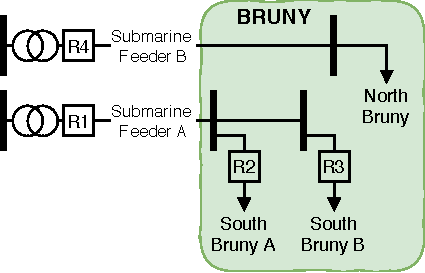
\includegraphics[width=.45\textwidth]{images/bruny_single_line.pdf}}
	\caption{Single line schematic of distribution network on Bruny Island.}
	\label{fig:bruny_network}
\end{figure}

\begin{figure}[htbp]
	\centerline{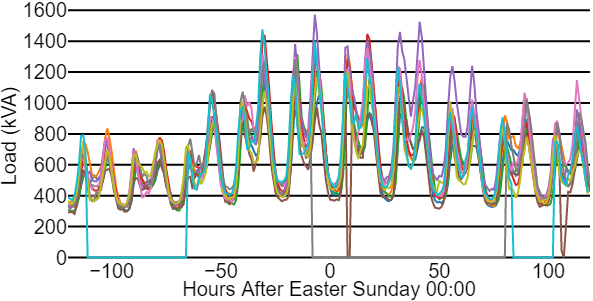
\includegraphics[width=.65\textwidth]{images/easter_bruny.png}}
	\caption{Easter load on Bruny Island 2008 through 2017.
		Unusable missing/bad data can also be seen in this graph.}
	\label{fig:bruny_easter}
\end{figure}

\subsection{Data analysis}
\label{bruny-data-analysis}

%\begin{itemize}
%	\item discuss available data - load, weather, cars, other feeders and reclosers
%	\item general load profiles of winter week, summer week, and full year
%	\item look at annual growth of electricity. I need to investigate further my graph that is anomalous for 2013 and 2014 in growth.
%	\item talk about different days of the week, and relate to car movement
%	\item Look at special days - easter, june, christmas/ny
%	\item talk about relationship between load and weather - temperature mainly
%	\item Is load influenced by humidity like literature claims, or are temperature and humidity simply related?
%	\item look at coloured scatter plot of load, temperature, and cumulative cars - more people correlates with more load in general - but we don't know future number of people.
%	\item correlation matrix for power, cars, and weather
%	\item cross correlations. Especially discuss any lags
%	\item perhaps conclude with some important takeaways
%\end{itemize}

In section \ref{patterns-profiles} the general properties of load profiles and how they are influenced by exogenous factors was discussed. Now, these general properties will be briefly investigated for the Bruny Island feeder.
\subsubsection{Available data}
The following data is available:
\begin{itemize}
	\item Apparent power measured at recloser R1 (figure \ref{fig:bruny_network}) between January 1, 2007 and June 25, 2018
	\item Ambient Temperature, solar irradiance, humidity, and wind speed at Lenah Valley between October 1, 2009 and June 25, 2018
	\item Vehicle movement data in 10 minute resolution between June 4, 2015 and March 24, 2018
\end{itemize}	
Vehicle movement data is provided as a set of observations every 10 minutes recording the number of vehicles arriving on the island, and the number of vehicles departing the island.
By integrating this, a relative number of vehicles on the island can be established.

There is a significant amount of bad or missing data throughout these datasets.
This has been handled by limiting the use of data where there are too many missing or bad values.

\subsubsection{Analysis}
Figure \ref{fig:load-profiles} shows apparent power draw on Bruny Island over a winter week, a summer week, and over an entire year.
These two weeks were selected to avoid special days such as holidays and are representative of typical weeks.
Several differences can be seen between the summer and winter weeks.
In Summer, the midday load is about the same as the overnight load, whereas in Winter, it is quite different.
Summer afternoon peaks are smaller than the morning peaks, whereas in winter they are similar.
At a high level, it is clear that the load is generally larger in winter -- likely as a result of increased residential heating.
An intuitive reaction to this might be to use different forecasting models for summer and winter - but of course then a delineation must be decided on for when to switch between the two models.
As one of the aims of the forecasting system is to be practical to implement, it is desirable to have a single system that is be able to forecast both summer and winter.
By supplying temperature as an exogenous input this should be possible.

\begin{figure}[htbp]
	\centering
	\subfigure[]{
		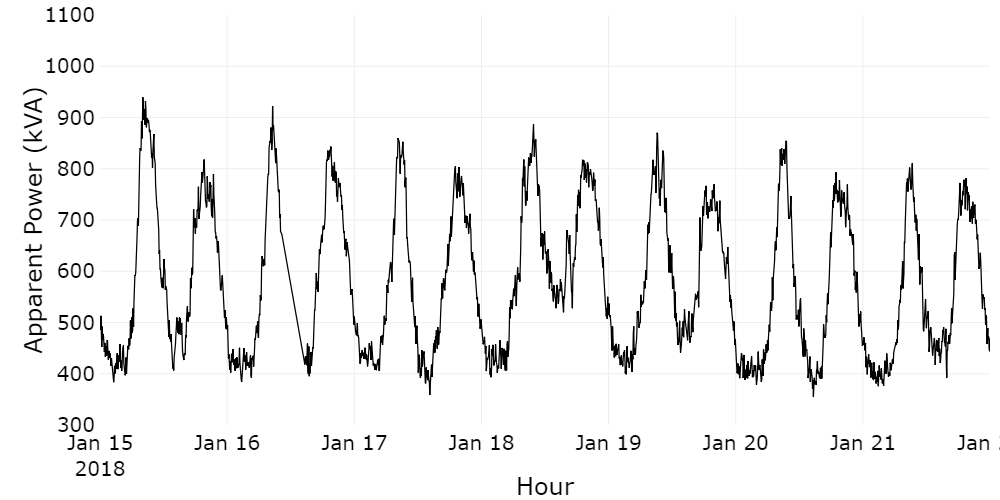
\includegraphics[width=0.8\textwidth]{images/simple-week-summer}
		\label{fig:simple-week-summer}}
	\vfil
	\subfigure[]{
		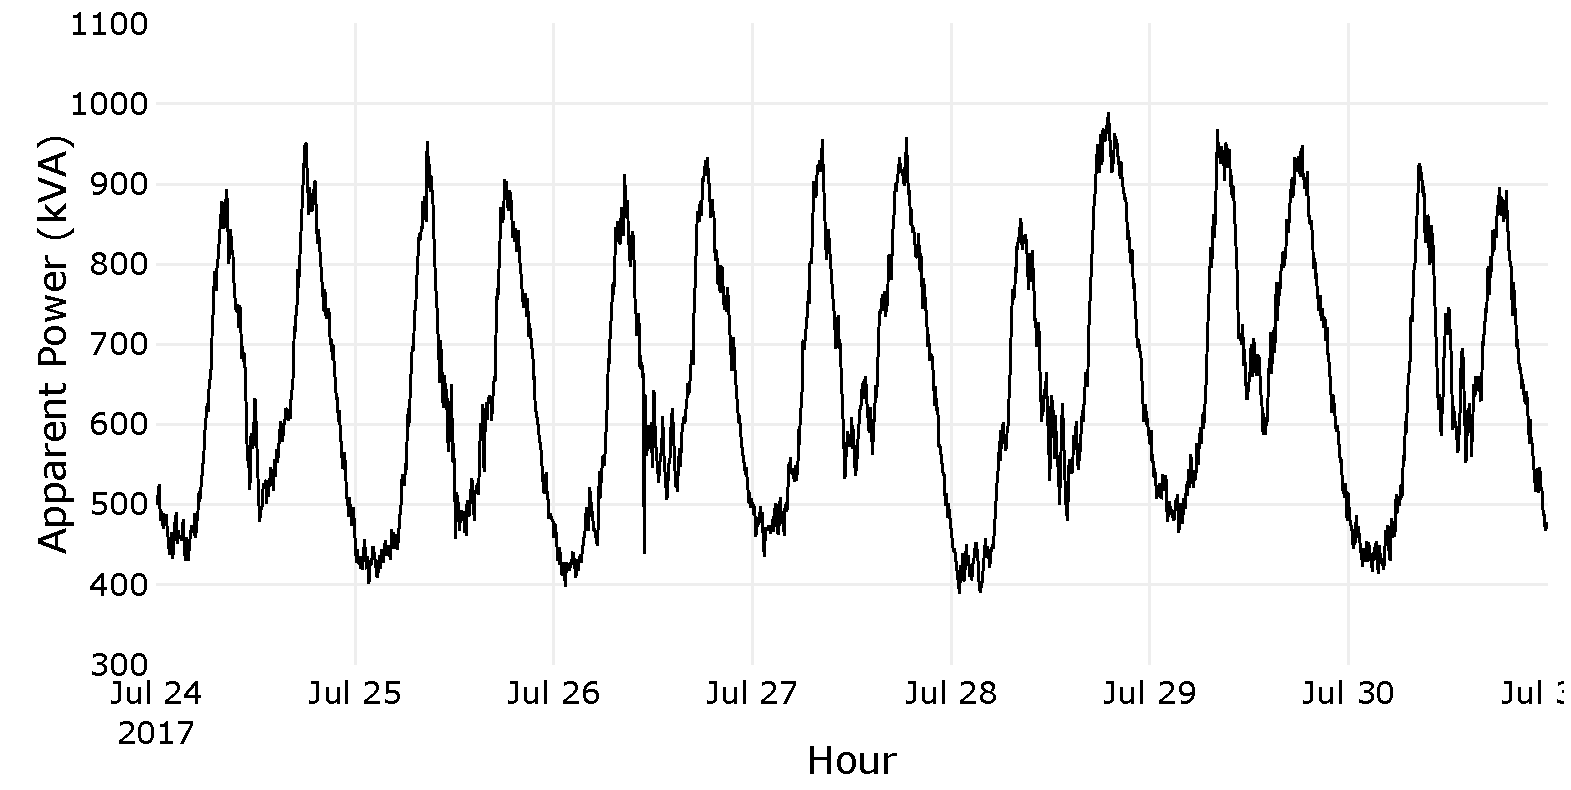
\includegraphics[width=0.8\textwidth]{images/simple-week-winter}
		\label{fig:simple-week-winter}}
	\vfil
	\subfigure[]{
		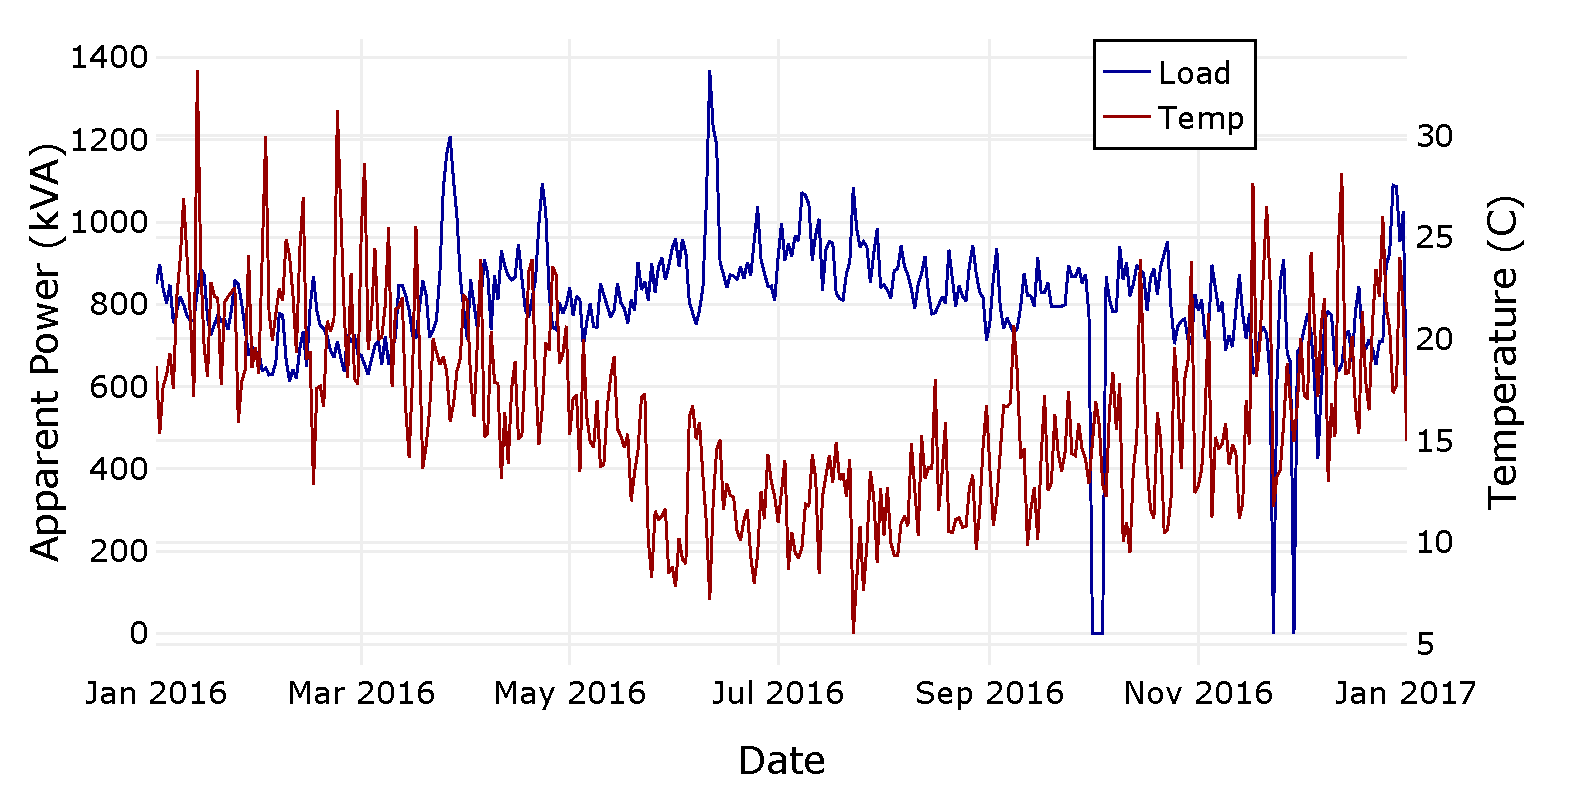
\includegraphics[width=0.8\textwidth]{images/max-load-max-temp}
		\label{fig:max-load-max-temp}}
	\caption{Bruny Island load profiles. (a) Load over a single summer week in 2018. (b) Load over a single winter week in 2017. (c) Peak daily load and peak daily temperature over all of 2017.}
	\label{fig:load-profiles}
\end{figure}

It was mentioned in section \ref{patterns-profiles} that weekends and weekdays tend to have different load profiles, but this is not immediately obvious from figure \ref{fig:load-profiles}.
Figure \ref{fig:average-profiles} shows this difference between days of the week.
What is immediately obviously is that the differences between days of the week are not restricted to 24 hour bounds - the different load profile shapes gently merge into each other over the course of an afternoon or morning.
% This is an especially important observation for a forecasting system that needs to be able to perform forecasts not just at a single time each day, but at any time.
It can be seen that the Friday profile morphs into the Saturday profile during the afternoon, perhaps as people arrive on the island for the weekend, and the Sunday profile morphs into a weekday profile over the afternoon, perhaps as people depart the island.

Figures \ref{fig:average-arriving} and \ref{fig:average-departing} further support that the changes in load profiles are a result of people arriving on or leaving the island.
It can be seen that many vehicles tend to arrive on the island on Friday afternoon, leading to the change in load profile between Friday and Saturday.
Likewise, many vehicles leave the island on Sunday afternoon, shifting the load profile from Sunday to a weekday.

This brief investigation serves to highlight some of the challenges that the load forecasting system must handle.

\begin{figure}[htbp]
	\centering
	\subfigure[]{
		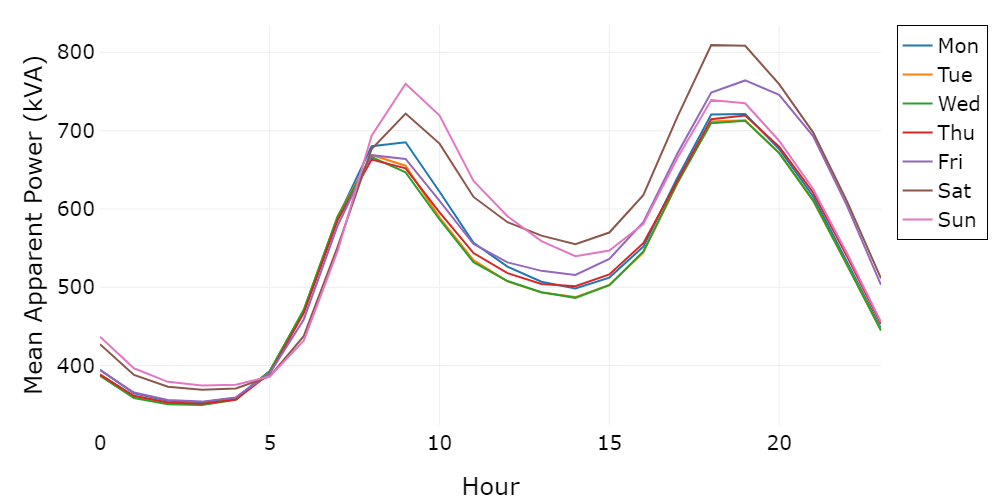
\includegraphics[width=.8\textwidth]{images/average-profiles}
		\label{fig:average-profiles}}
	\vfil
	\subfigure[]{
		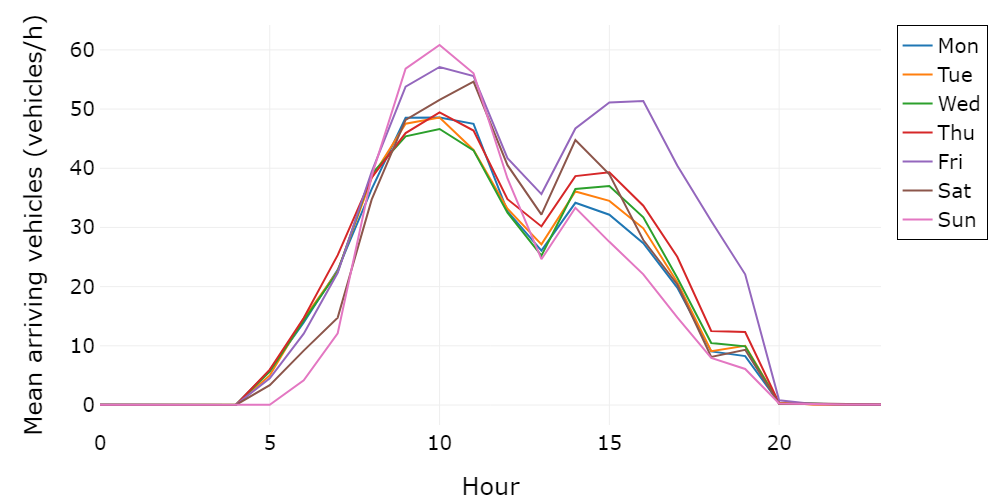
\includegraphics[width=.8\textwidth]{images/average-arriving}
		\label{fig:average-arriving}}
	\vfil
	\subfigure[]{
		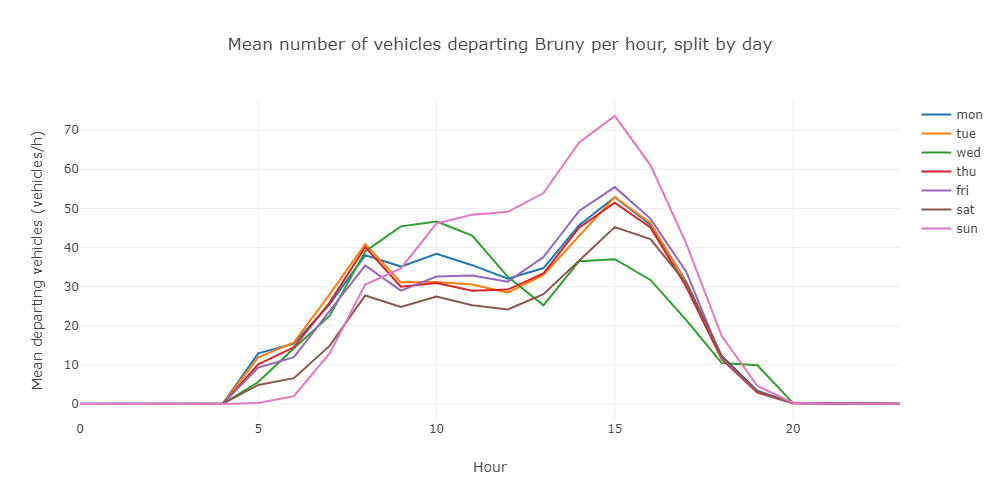
\includegraphics[width=.8\textwidth]{images/average-departing}
		\label{fig:average-departing}}
	\caption{Bruny Island average load profiles. (a) Average load profiles for each day of the week. Average number of cars arriving on (b) and leaving (c) the island each day.}
	\label{fig:average-load-profiles}
\end{figure}

\subsection{Forecasting tasks}
The forecasters were evaluated on several tasks, shown in table \ref{table:offline-results-bruny-lscape}.
The hourly task has the forecaster predict the future 24 hours of load in one-hour resolution given the previous 24 hours of load and the future 24 hours of date/time, holiday, and temperature data.
The half-hourly task is the same as hourly, except using half-hour resolution data.
The hourly long task has the forecaster predict the future 24 hours of load in one-hour resolution given the previous 168 hours (one week) of load and the future 24 hours of date/time, holiday, and temperature data.
The hourly ($c$=3) task is the same as the hourly task but with the loss function modified as described in section \ref{train-reg}.

The tasks listed as being ''with similar profiles" include five similar profiles ($k=5$, as described in the following section \nameref{data-model-config}).
The tasks that do not list similar profiles have no similar profiles, $k=0$.

\subsection{Data and  model configuration}
\label{data-model-config}
The available data was split into a training set (October 1 2009 through February 15 2014) and a testing set (February 16 2014 through June 25 2018).
For the hourly task, the network was supplied with data in hourly resolution from the previous and future 24 hours:
\begin{itemize}
	\item The previous 24 hours of load, $\vl = [ l_1 \: l_2 \: ...  \: l_{24}]^\top$, with $l_{24}$ being the most recent load.
	\item Temperature for the future 24 hours, $\vt = [t_1 \: t_2 \: ... \: t_{24}]^\top$, with $t_1$ being the soonest point in the future.
	\item Day of the week as an integer from 0 to 6 (local time) over the future 24 hours, $\vd = [d_1 \: d_2 \: ... \: d_{24}]^\top$, with $d_1$ being the soonest point in the future.
	\item Minutes since midnight (local time) for the future 24 hours, $\vm = [m_1 \: m_2 \: ... \: m_{24}]^\top$, with $m_1$ being the soonest point in the future.
	\item Boolean 1 or 0 indicating whether it is a holiday at each hour over the next 24 hours, $\vh = [h_1 \: h_2 \: ... \: h_{24}]^\top$, with $h_1$ being the soonest point in the future.
	\item Holiday type as an integer from 0 to $n$ at each hour over the future 24 hours, where there are $n$ different holidays in the year, $\vg = [g_1 \: g_2 \: ... \: g_{24}]^\top$, with $g_1$ being the soonest point in the future.
	\item Month of the year from 0 to 11 (local time) over the future 24 hours, $\vn = [n_1 \: n_2 \: ... \: n_{24}]^\top$, with $n_1$ being the soonest point in the future.
\end{itemize}

Additionally, similar profile data was constructed for $k$ similar days, as described in section \ref{simperiod}.
The weights used are given in table \ref{table:offline-parameters}.
The extremely large weights are used to ensure that similar profiles are always selected from the same month and day of month/day of week unless there are none available.
The similar day data is aligned with the same points in time as the $\vt$ vector (and others).
The similar profile data is:

\begin{itemize}
	\item 24 hours of similar profile load $\vl_{sk} = [ l_{sk1} \: l_{sk2} \: ... \: l_{sk24}]^\top$.
	\item 24 hours of similar profile temperature, corresponding to the same points in time as $\vl_{sk}$, $\vt_{sk} = [ t_{sk1} \: t_{sk2} \: ...  \: t_{sk24}]^\top$.
\end{itemize}

This data was concatenated to form the input matrix given in equation \ref{eq:input-matrix}.

\begin{equation} \label{eq:input-matrix}
\mX = [ \vl \: \vt \: \vd \: \vm \: \vh \: \vg \: \vn \: \vl_{s1} \: \vt_{s1} \: \ldots \: \vl_{sk} \: \vt_{sk}] \in \mathbb{R}^{24 \times (7 + 2k)}
\end{equation}

The half-hourly configuration is the same as the hourly configuration, except all vectors contain 48 elements (representing 24 hours of data) and so $\mX \in \mathbb{R}^{48 \times (7 + 2k)}$.

The hourly long configuration modifies only the $\vl$ vector, such that $\vl = [ l_1 \: l_2 \: ...  \: l_{168}]^\top$ representing one week of hour-resolution data, with $l_{168}$ being the most recent observation.
The other vectors were zero padded to match this length.
With $\vz \in \mathbb{R}^{144}$ being a zero vector, and $\hat{\vv} = [\vz^\top \vv^\top]^\top$ for any vector $\vv$, the input $\mX$ is given by
\begin{equation}
\mX = [ \hat{\vl} \: \hat{\vt} \: \hat{\vd} \: \hat{\vm} \: \hat{\vh} \: \hat{\vg} \: \hat{\vn} \: \hat{\vl_{s1}} \: \hat{\vt_{s1}} \: \ldots \: \hat{\vl_{sk}} \: \hat{\vt_{sk}}] \in \mathbb{R}^{168 \times (7 + 2k)}
\end{equation}

The forecasting models were configured with the parameters given in table \ref{table:offline-parameters} and trained for $10^5$ iterations.
All the models presented in section \ref{ana-meth} are evaluated.
The ``Transformer" model is the transformer with teacher forcing enabled, and the ``Transformer no TF" model is the transformer with teacher forcing disabled.

\begin{table}[htbp]
	\caption{Offline Evaluation model parameters.}
	\begin{center}
	\begin{tabular}{lclc}
	\multicolumn{1}{c}{\textbf{Model/Method}} & \textbf{Parameter} & \textbf{Description}                 & \textbf{Value} \\ \cline{1-4} 
	
	\multirow{6}{*}{\shortstack[l]{SARIMAX}}       
	& $p$                & AR model order     					& 2              \\
	& $d$                & Number of differences   		        & 1             \\
	& $q$                & MA model order           			& 1              \\
	& $P$                & Seasonal AR model order              & 1            \\
	& $D$                & Number of seasonal differences       & 1              \\
	& $Q$                & Seasonal MA model order              & 1             \\
	& $s$                & Period of seasonality		        & 24             \\ \cline{1-4} 
	
	\multirow{6}{*}{\shortstack[l]{Sequence to\\Sequence}}       
	& $L$                & Number of encoder and decoder layers & 2              \\
	& $d$                & Hidden dimension                     & 16             \\
	& $D$                & Dropout fraction                     & 0            \\
	& $c$                & Loss function modifier               & 0              \\
	& $l$                & Learning rate 			            & 0.001             \\
	& -                  & Training batch size                  & 16             \\ \cline{1-4} 
	
	\multirow{6}{*}{\shortstack[l]{Transformer}}       
	& $L$                & Number of encoder and decoder layers & 2              \\
	& $d$                & Hidden dimension                     & 16             \\
	& $h$                & Number of attention heads            & 2              \\
	& $D$                & Dropout fraction                     & 0.2            \\
	& $c$                & Loss function modifier               & 0              \\
	& $l$                & Learning rate 			            & 0.001              \\
	& -                  & Training batch size                  & 16             \\ \cline{1-4} 
	
	\multirow{6}{*}{\shortstack[l]{Universal Transformer}}      
	& $L$                & Number of encoder and decoder layers & 2              \\
	& $d$                & Hidden dimension                     & 16             \\
	& $h$                & Number of attention heads            & 2              \\
	& $D$                & Dropout fraction                     & 0.2            \\
	& $c$                & Loss function modifier               & 0              \\
	& $l$                & Learning rate 			            & 0.001              \\
	& -                  & Training batch size                  & 16             \\ \cline{1-4} 
	
	\multirow{6}{*}{\shortstack[l]{Similar\\Profile\\Selection}}
	& -                  & Maximum future temperature weight    & 10             \\
	& -                  & Minimum future temperature weight    & 20             \\
	& -                  & Maximum past load weight             & 30             \\
	& -                  & Holiday type weight                  & 1e9            \\
	& -                  & Day of week weight                   & 1e6            \\
	& -                  & Day of month weight                  & 1e6            \\
	& -                  & Month of year weight                 & 1e6           
\end{tabular}
		\label{table:offline-parameters}
	\end{center}
\end{table}


\subsection{Offline evaluation results}
The forecaster was trained on the training dataset (October 1 2009 through February 15 2014) and tested on the testing dataset (February 16 2014 through June 25 2018).
The train and test datasets were then switched in order to cross-validate the results.
All presented results are the average of the cross validated results.
Results are shown in table \ref{table:offline-results-bruny-lscape}.

Both the mean absolute percentage error (MAPE) and mean absolute error (MAE) are shown.
These metrics are calculated for all load, for load only over 1MVA, and for load that is at a first large peak.
A first large peak is a morning or afternoon peak that is over 1MVA and is greater than 36 hours after any previous peak that was over 1MVA.
The first large peak metric is used because it is generally considered difficult to forecast.
These two metrics allow the performance of the system on anomalous holiday periods to be more directly evaluated.

The SARIMAX model proved to produce results that are relatively poor compared to the other models, and so was not considered beyond the hourly without similar days task.
The universal transformer is consistently a poor performer, never producing the best results for any task or metric.
The transformer model is generally outperformed by, or very similar to, the transformer without teacher forcing.

Looking at the results table, it is clear that there is no model which is overall superior between the sequence to sequence and transformer without teacher forcing models.

The sequence to sequence model appears to excel at the hourly task achieving the best MAPE scores above 1 MVA and at first large peak, while also being close to the transformer without teacher forcing on the overall MAPE score.

The transformer without teacher forcing is generally good at minimizing the overall MAPE score.
It also performs exceedingly well in the hourly long task, achieving the lowest overall MAPE while the other two metrics are close to the hourly with similar and $c=3$ task.
This model is also arguably the best at the half-hourly tasks, achieving the best results on the majority of metrics across both tasks. 

The hourly with $c=3$ tasks show no consensus on which model is generally superior.


\afterpage{%
	\clearpage% Flush earlier floats (otherwise order might not be correct)
	\thispagestyle{empty}% empty page style (?)
	\begin{landscape}% Landscape page
		\centering % Center table
		\begin{table}[htbp]
			\caption{Offline evaluation results.}
			% \begin{center}
				\begin{tabular}{llcccccc}
					\multicolumn{1}{c}{\textbf{Task}} &
					\multicolumn{1}{c}{\textbf{Model}} & 
					\multicolumn{1}{c}{\textbf{\shortstack[c]{MAPE\\(\%)}}} &
					\multicolumn{1}{c}{\textbf{\shortstack[c]{MAE\\(kVA)}}} & 
					\multicolumn{1}{c}{\textbf{\shortstack[c]{MAPE over\\1 MVA (\%)}}} &
					\multicolumn{1}{c}{\textbf{\shortstack[c]{MAE over\\1 MVA (kVA)}}} &
					\multicolumn{1}{c}{\textbf{\shortstack[c]{MAPE at first\\large peak (\%)}}} &
					\multicolumn{1}{c}{\textbf{\shortstack[c]{MAE at first\\large peak (kVA)}}} \\ \cline{1-8}
					
					\multirow{4}{*}{\shortstack[l]{Hourly}}       
					& SARIMAX           &         14.34  &         82.1  &         12.31  &         137.7  &         18.86  &         200.9 	\\ % (2,1,1)(1,1,1,24)/_cv
					& S2S      			&          7.85  &         42.8  &  \textbf{9.87} & \textbf{110.6} & \textbf{11.42} & \textbf{112.6}	\\ % 
					& Transformer       &          7.82  &         43.1  &         10.33  &         115.1  &         13.00  &         140.1 	\\ % 
					& Transformer no TF &  \textbf{7.77} & \textbf{42.6} &         11.45  &         128.9  &         13.24  &         142.0 	\\ % 130 131
					& U. Transformer    &          8.20	 &         46.0  &         11.72  &         131.6  &         14.52  &         155.2 	\\ % 
					\cline{1-8}					
					
					\multirow{3}{*}{\shortstack[l]{Hourly\\with similar\\profiles}} 
					& S2S      			&          7.68  &         41.6  &  \textbf{9.77} & \textbf{109.6} & \textbf{11.05} & \textbf{118.7}	\\ % 
					& Transformer       &          7.40  &         40.7  &         10.25  &         115.2  &         12.45  &         133.6 	\\ % 
					& Transformer no TF &  \textbf{7.24} & \textbf{39.6} &         10.32  &         115.8  &         12.47  &         133.7    	\\ % 122 123
					& U. Transformer    &          8.15  &         44.8  &         11.10  &         123.5  &         12.67  &         135.5 	\\ % 
					\cline{1-8}					
					
					\multirow{3}{*}{\shortstack[l]{Half-\\hourly}}       
					& S2S      			&  \textbf{7.80} & \textbf{42.7} &          9.88  &         111.3  &         12.30  &         131.5 	\\ % 
					& Transformer       &          9.14  &         50.9  &         13.03  &         148.0  &         15.80  &         170.0 	\\ % 
					& Transformer no TF &          8.24  &         44.0  &  \textbf{9.03} & \textbf{101.5} & \textbf{10.22} & \textbf{110.4}  	\\ % 126 127
					& U. Transformer    &          8.60  &         48.0  &         13.60  &         154.6  &         14.33  &         154.5 	\\ % 
					\cline{1-8}					
					
					\multirow{3}{*}{\shortstack[l]{Half-hourly\\with similar\\profiles}}       
					& S2S      			&          8.44  &         45.0  &         10.23  &         116.2  &         11.10  &         119.1 	\\ % 
					& Transformer       &          7.82  &         42.5  &         10.78  &         121.6  & \textbf{10.98} & \textbf{118.5}	\\ % 
					& Transformer no TF &  \textbf{7.41} & \textbf{41.0} & \textbf{10.16} & \textbf{114.1} &         12.54  &         134.8  	\\ % 128 129
					& U. Transformer    &          9.05  &         48.1  &         10.22  &         114.6  &         11.90  &         136.0 	\\ % 
					\cline{1-8}					
					
					\multirow{3}{*}{\shortstack[l]{Hourly long\\with similar\\profiles}}       
					& S2S      			&          7.49  &         40.9  &  \textbf{9.43} & \textbf{106.2} &         10.10  &         109.5 	\\ % 
					& Transformer       &          6.97  &         38.0  &         10.82  &         122.5  &         11.30  &         121.8 	\\ % 
					& Transformer no TF &  \textbf{6.68} & \textbf{36.8} &          9.85  &         111.8  &  \textbf{9.54} & \textbf{103.1} 	\\ % 132 133
					& U. Transformer    &          6.74  &         38.5  &         10.35  &         116.1  &         12.82  &         138.2 	\\ % 
					\cline{1-8}					
					
					\multirow{3}{*}{\shortstack[l]{Hourly; $c=3$}}       
					& S2S      			&          8.96  &         46.8  &  \textbf{8.61} &  \textbf{95.9} &  \textbf{9.61} & \textbf{103.0}	\\ % 
					& Transformer       &  \textbf{8.14} & \textbf{44.5} &         10.46  &         117.5  &         12.25  &         130.9 	\\ % 
					& Transformer no TF &          8.65  &         45.4  &          9.36 &          105.0  &         10.76  &         115.1  	\\ % 134 135
					& U. Transformer    &          9.29  &         48.5  &         11.05  &         124.5  &         12.97  &         138.9 	\\ % 
					\cline{1-8}					
					
					\multirow{3}{*}{\shortstack[l]{Hourly\\with similar\\profiles; $c=3$}}       
					& S2S      			&  \textbf{8.32} & \textbf{43.8} &          9.20  &         103.1  &         10.68  &         114.8 	\\ % 
					& Transformer       &          8.58  &         45.5  &  \textbf{8.90} &  \textbf{99.5} &  \textbf{9.29} &  \textbf{99.9}	\\ % 
					& Transformer no TF &          8.86  &         45.4  &          8.99  &         101.1  &         10.21  &         109.7  	\\ % 136 137
					& U. Transformer    &          9.00  &         48.3  &         10.07  &         112.5  &          9.34  &         100.5 	\\ % 
					\cline{1-8} 
				\end{tabular}
				\label{table:offline-results-bruny-lscape}
			% \end{center}
		\end{table}
	\end{landscape}
	\clearpage% Flush page
}


\subsection{Training data requirements}
Neural networks generally require large amounts of training data in order to fit the model parameters.


\subsection{Online CONSORT implementation}
\label{consort-eval}
In July 2018 the load forecasting system was implemented as part of the CONSORT project.
The forecasting system was used to assist with dispatch of residential batteries.
The model implemented was a transformer (with teacher forcing enabled), and is somewhat different to the models discussed in the offline evaluation.
Although the implemented model achieved sufficient accuracy, it has since been determined to be a sub-optimal configuration.


\subsubsection{Data and  Model Configuration}
The following data was available from 2009-2018:
\begin{itemize}
	\item Apparent power at reclosers R1 through R4 (Figure \ref{fig:bruny_network}).
	\item Temperature at Lenah Valley, Tasmania (50km from Bruny Island). 
	\item Apparent power consumption at St Helens, Tasmania.
\end{itemize}

This data was averaged to 30 minute resolution and split into a training set containing data from October 2009 through September 2014, and a testing set containing data from October 2014 through April 2018.

The network was supplied with data from the previous and future 24 hours, for a total input sequence length of 96 (representing 48 hours at 30 minute resolution).
The output sequence length was 48 (24 hours).

The following time series were supplied to the model input:
\begin{itemize}
	\item Apparent power from recloser R1 (Figure \ref{fig:bruny_network}), with future values set to zero.
	\item Temperature.
	\item Day of the week as an integer from 0 to 6 (local time).
	\item Minutes since midnight (local time).
	\item Boolean 1 or 0 indicating whether it is a holiday.
	\item Holiday type.
\end{itemize}

When used for inference, temperature forecasts were obtained from the Bureau of Meteorology.

Additionally, five similar periods were identified using data from R1 by the process described in section \ref{simperiod}.
The data over the similar periods for each of the following time series was provided as input:
\begin{itemize}
	\item Reclosers R1, R2, R3, and R4 (Figure \ref{fig:bruny_network}) (as separate time series).
	\item St Helens recloser.
	\item Lenah Valley temperature.
\end{itemize}

In total, 36 time series were provided as input to the model.
St Helens was included because it was observed to display similar patterns to Bruny Island around holiday periods.

The forecasting system was configured with the parameters in table \ref{table:parameters}, with the upper section giving transformer model parameters and the lower section giving weights used for similar period selection.
The model was trained for $10^5$ iterations.

\begin{table}[htbp]
	\caption{Case study model parameters.}
	\begin{center}
		\begin{tabular}{clc}
			%			3.\hline
			\textbf{Parameter}&\textbf{Description}&\textbf{Value} \\
			\hline
			$L$ & Number of encoder and decoder layers & 4 \\
			$d$ & Hidden dimension & 32 \\
			$h$ & Number of attention heads & 4 \\
			$D$ & Dropout fraction & 0.2 \\
			$c$ & Loss function modifier & 3 \\
			-   & Training batch size & 16 \\
			\hline
			-   & Maximum future temperature weight & 10 \\
			-   & Minimum future temperature weight & 20 \\
			-   & Maximum past load weight & 30 \\
			-   & Holiday type weight & 1e9 \\
			-   & Day of week weight & 1e6 \\
			-   & Day of month weight & 1e6 \\
			-   & Month of year weight & 1e6 \\
			
		\end{tabular}
		\label{table:parameters}
	\end{center}
\end{table}

%\subsubsection{Offline Evaluation}
%
%The forecaster was first evaluated on historical data around Easter 2018, shown in Figure \ref{fig:easter_forecasts}.
%Notably, the forecaster was able to accurately predict the first large peak while also transitioning smoothly between normal and holiday periods.
%This is in contrast to load forecasting models which sometimes tend toward trivially repeating the previous day's load.
%
%
%\begin{figure}[htbp]
%	\centerline{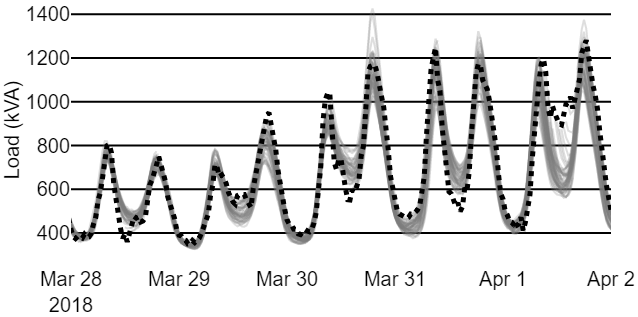
\includegraphics[width=.65\textwidth]{images/easter_2018_all_forecast.png}}
%	\caption{Forecasts over the Easter 2018 period.
%		The black dashed line is the actual recorded load, and all previous forecasts are shown in grey.}
%	\label{fig:easter_forecasts}
%\end{figure}
%
%\begin{figure}[htbp]
%	\centerline{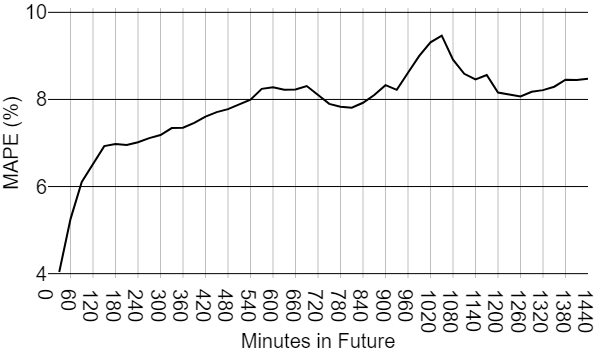
\includegraphics[width=.65\textwidth]{images/bruny_mape.png}}
%	\caption{Mean absolute percentage error of each point in the forecast when evaluated over a variety of holiday periods.}.
%	
%	\label{fig:bruny_mape}
%\end{figure}
%
%The performance of the forecaster was evaluated on every Easter, Queen's Birthday, and July school holiday period from 2015 through 2018 (2018 excludes July).
%The results are shown in Figure \ref{fig:bruny_mape}, showing the mean absolute percentage error (MAPE) as a function of forecast horizon.
%The mean MAPE is 7.4\%.
%Furthermore, the errors between predicted and actual load are fairly evenly distributed around -15 kVA, shown in Figure \ref{fig:bruny_hist}.
%This indicates that the model has some room for improvement when predicting large holiday peaks, but overall this is evidence that the model has been able to generalize from the training data, as the training data is mostly comprised of normal days.
%
%\begin{figure}[htbp]
%	\centerline{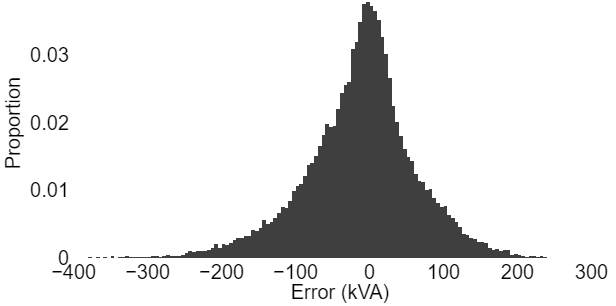
\includegraphics[width=.65\textwidth]{images/errors_histogram.png}}
%	\caption{Distribution of forecast error when evaluated over the same periods as Figure \ref{fig:bruny_mape}.}
%	\label{fig:bruny_hist}
%\end{figure}

\subsubsection{Online Evaluation}
When implemented live on the Bruny Island distribution network during the July 2018 school holiday period, as part of the CONSORT project, the forecaster was observed to reliably forecast large demand peaks.
This enabled the fleet of distributed batteries to be used effectively in providing network support via net demand peak reduction. An accurate forecast, issued early enough in advance of the occurence of the demand peak, was observed to give the batteries adequate time to store energy in the lead up to, and discharge during the demand peak period. In at least one instance over the test period this was sufficient to avoid the island's diesel generator from being used at all, when it otherwise almost certainly would have been required.
Data collected during this peak demand period can be seen in Figure \ref{fig:bruny_nac}.
The upper section shows 24 hours of historical load in black, plus the most recent 24-hour horizon forecast in dashed black (recalculated every five minutes) and all old forecasts in grey.
The lower section shows the battery charge rate, where a negative value of battery charge rate indicates the batteries are supporting the grid.

Typically the generator is switched on when load exceeds 1050 kVA.
During the first peak the graph shows the batteries supplying between 50 and 100 kW to the island.
Without this support from the batteries, the generator would have been required to operate.

\begin{figure}[htbp]
	\centerline{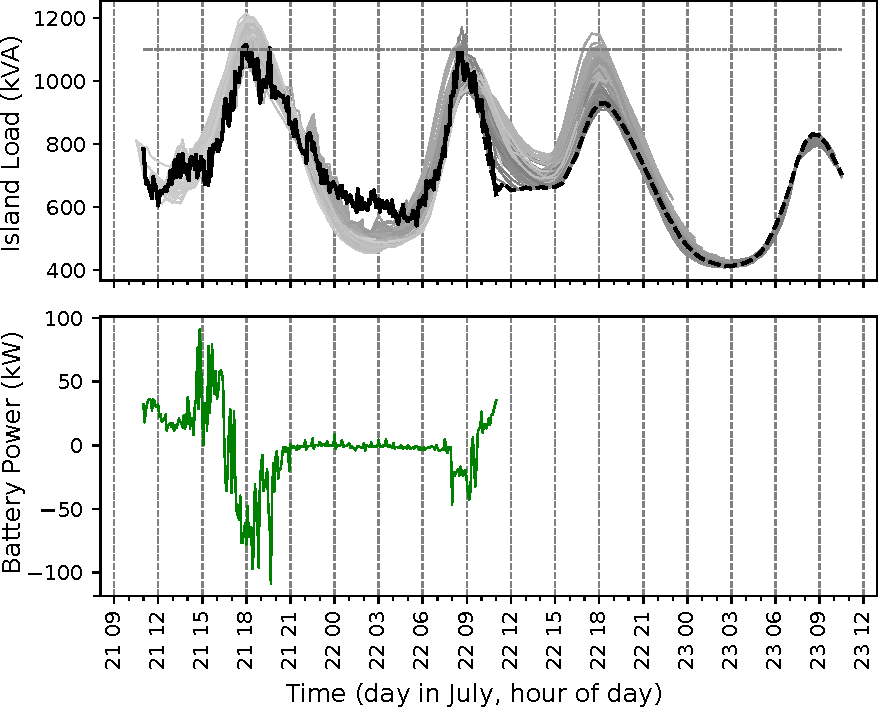
\includegraphics[width=.65\textwidth]{images/bruny_nac.pdf}}
	\caption{Results from the forecasting system's implementation in the CONSORT project.}
	\label{fig:bruny_nac}
\end{figure}




